% 原书 p.52–p.55（PDF p.60–p.63）
\chapter{切触几何（Contact Geometry）}

切触几何与辛几何颇为相似，研究的是奇数维光滑流形上的切触结构。切触结构最初出现于
偏微分方程的研究之中；尽管它相当受限，却在自然界的种种现象中屡屡现身。经过多年发展，
切触几何如今已与众多领域相互联系，尤其在低维拓扑中。本章除介绍切触几何的基本背景之外，
将着重讨论若干与辛几何中相应概念平行对应的概念。

\section{切触结构（Contact Structure）}

\begin{keytakeaways}
\begin{itemize}
  \item 几何图像：切触结构是奇数维流形上「完全不可积」的超平面场，其非退化性由
        $\alpha\wedge(\dd\alpha)^n\neq 0$ 刻画，恰与 Frobenius 可积性条件
        $\alpha\wedge(\dd\alpha)^n\equiv 0$ 相反。
  \item 数学工具：切触 $1$-形式、Reeb 向量场 $R_\alpha$（由
        $\dd\alpha(R_\alpha,\cdot)=0$、$\alpha(R_\alpha)=1$ 唯一确定）、
        规范变换 $\alpha\mapsto e^f\alpha$，以及 $\dd\alpha|_\xi$ 给出的
        「共形辛结构」。
  \item 本节结论：切触流形必可定向（可余定向时）；Reeb 流保持 $\alpha$，从而是严格
        切触同胚；切触几何的核心问题是 Weinstein 猜想——闭切触流形上 Reeb 流必有闭轨道。
\end{itemize}
\end{keytakeaways}

% >>> p060
给定一个 $(2n+1)$ 维光滑流形 $M^{2n+1}$。$M$ 上的一个\textbf{超平面场}
（hyperplane field）是指在每一点 $x\in M$ 处指定一个 $2n$ 维平面
$\xi_x\subset T_xM$ 的光滑分布。$M$ 上每个超平面场 $\xi$ 都局部地由一个
$1$-形式的核给出：确切地说，对每点 $x\in M$，都存在邻域 $U_x$ 以及定义在
$U_x$ 上的 $1$-形式 $\alpha$，使得 $\xi|_{U_x}=\ker\alpha$。考虑 $M$ 上的
秩一向量丛 $TM/\xi$。若它是平凡的，即含有非零截面，则称 $\xi$ 是
\textbf{可余定向的}（co-oriented）。此时可找到整体定义的 $1$-形式 $\alpha$，
使 $\xi=\ker\alpha$。本章为简单起见，总假定 $\xi$ 可余定向。

\begin{wdefn}{3.1.1}
设 $M^{2n+1}$ 是一个 $(2n+1)$ 维流形。其上的（可余定向）\textbf{切触结构}
（contact structure）是一个超平面场 $\xi$，满足 $\xi=\ker\alpha$，并具有如下
非退化条件：
\begin{equation}\tag{3.1}
  \bigl(\alpha\wedge(\dd\alpha)^n\bigr)_x\neq 0
\end{equation}
对任意 $x\in M$ 成立。这里任何这样的 $\alpha$ 都称为 $\xi$ 的
\textbf{切触 $1$-形式}（contact $1$-form）。\textbf{切触流形}
（contact manifold）是指二元组 $(M^{2n+1},\xi)$，其中 $\xi$ 是 $M$ 上的
切触结构。
\end{wdefn}

% [Tutor Note: 易错预警——非退化条件 (3.1) 是逐点的 $(2n+1)$-形式非零条件。
% 由于 $(2n+1)$-形式空间一维，它等价于
% $\alpha\wedge(\dd\alpha)^n$ 为体积形式；又因若 $\alpha$ 在某点为零则楔积必为零，
% 故条件自动蕴含 $\alpha$ 处处非零，从而 $\ker\alpha$ 是真正的 $2n$ 维分布。
% 另注意 $(\dd\alpha)^n$ 指 $\dd\alpha$ 的 $n$ 次楔积，并非外微分作用 $n$ 次。]

% [Tutor Note: 易错预警——「可余定向」在原文中也称 co-oriented。若 $TM/\xi$ 非平凡
% （例如 $\xi$ 为不可定向流形上的切触超平面场），则 $\alpha$ 只能局部选取，切触
% $1$-形式无整体定义；此时 (3.1) 应逐局部理解。定义 3.1.1 中的整体 $\alpha$ 与
% 「可余定向」互为等价，不可混为一谈。]

回忆：$M^{2n+1}$ 上的超平面场 $\xi$ 作为分布是可积的，当且仅当对任意
$p\in M$，局部存在子流形 $N$ 使得 $T_pN=\xi_p$。由 Frobenius 可积性定理
（见 [239] 中的命题 1.59、定理 1.60 以及命题 2.30），该条件等价于
$\alpha\wedge(\dd\alpha)^n\equiv 0$。由定义 3.1.1 中的 (3.1)，切触结构处处
非零，远非可积——它通常被称为\textbf{完全不可积的}
（completely non-integrable）！

% [Tutor Note: 含糊点拨——Frobenius 定理给出的是三件等价事的链条：
% $\xi$ 可积 $\iff$ $\dd\alpha|_\xi\equiv 0$ $\iff$ $\alpha\wedge(\dd\alpha)^n\equiv0$
% （第一个等价是 Frobenius 定理，第二个用到 $\xi=\ker\alpha$）。切触条件恰恰说
% $\dd\alpha|_\xi$ 处处非退化，是「最大程度地不可积」。核对时务必分清
% $\dd\alpha$ 的 $\xi$-分量与它在 $R_\alpha$ 方向的分量。]

% >>> p061
对给定的切触结构 $\xi$，切触 $1$-形式 $\alpha$ 并不唯一确定。把 $\alpha$
换成 $e^f\alpha$（$f:M\to\R$ 光滑），得到同一 $\xi$ 的另一切触 $1$-形式，
因为
\[
  (e^f\alpha)\wedge\bigl(\dd(e^f\alpha)\bigr)^n
  =(e^f)^{n+1}\alpha\wedge(\dd\alpha)^n
\]
仍满足定义 3.1.1 中的非退化条件 (3.1)。反之，任何生成切触结构 $\xi$ 的切触
$1$-形式必形如 $e^f\alpha$。有时我们记 $(M,\xi=\ker\alpha)$，以强调已选定或
固定了切触结构 $\xi$ 的某个切触 $1$-形式 $\alpha$。

由定义 3.1.1 直接可得若干初等观察。

(i) 若 $(2n+1)$ 维流形 $M^{2n+1}$ 容许（可余定向）切触结构
$\xi=\ker\alpha$，则 $M$ 可定向，因为 $\alpha\wedge(\dd\alpha)^n$ 给出一个
体积形式。

\begin{wrem}{3.1.1}
若考虑 $M$ 上更一般的切触结构（不必可余定向），则 $M$ 的可定向性不再是
必要条件。例如，$M=\R^3\times\RP^2$ 作为不可定向流形容许一个切触结构
（见 [92] 中例 2.1.11）。
\end{wrem}

(ii) 对切触流形 $(M,\xi)$ 上固定的切触 $1$-形式 $\alpha$，存在唯一的
向量场 $R_\alpha$ 满足如下方程组：
\begin{equation}\tag{3.2}
  \dd\alpha(R_\alpha,\cdot)=0,\qquad \alpha(R_\alpha)=1.
\end{equation}
(3.2) 中第一个条件大致是说向量场 $R_\alpha$「正交」于 $\xi$，而第二个条件
则对此向量场作归一化（从而唯一确定它）。

为证明 $R_\alpha$（满足 (3.2)）的存在性，注意 $TM$ 上的 $2$-形式
$\dd\alpha$ 逐点必有非零核，理由是关于维数的：确切地说，存在光滑向量场
$X$ 使得 $\dd\alpha(X,\cdot)=0$。由于 $\alpha\wedge(\dd\alpha)^n$ 逐点
非零，有 $\alpha(X)\neq0$。于是把 $X$ 重新缩放，即得所求的向量场
$R_\alpha$。向量场 $R_\alpha$ 称为 $\alpha$ 的 \textbf{Reeb 向量场}
（Reeb vector field）。

% [Tutor Note: 易错预警——$R_\alpha$ 依赖 $\alpha$ 的选取与符号约定：把
% $\alpha$ 换成 $-\alpha$ 时 $R_{-\alpha}=-R_\alpha$；换成 $e^f\alpha$ 时，
% $R_{e^f\alpha}=e^{-f}(R_\alpha+X_f)$，其中 $X_f\in\xi$ 由
% $\dd\alpha(X_f,Y)=\dd f(Y)$（$\forall Y\in\xi$）唯一确定（因为 $\dd\alpha|_\xi$
% 非退化）。教材取 $\alpha(R_\alpha)=1$ 这一特定归一化，与 §3.5 中接触哈密顿
% 向量场的符号约定必须对照阅读。]

下面的练习表明，Reeb 向量场的表达式对切触 $1$-形式的选择很敏感。

\begin{wexer}{3.1.1}
给定切触流形 $(M,\xi=\ker\alpha)$ 以及 $M$ 上的光滑函数 $f$，设
$\beta=e^f\alpha$ 是 $M$ 上的切触形式。试用 $\alpha$ 的 Reeb 向量场
$R_\alpha$ 表示 $\beta$ 的 Reeb 向量场。（提示：利用下文 (iv)。）
\end{wexer}

% [Tutor Note: 含糊点拨——本题的实质是：设 $R_\beta=e^{-f}(R_\alpha+X_f)$，
% 用 $\beta(R_\beta)=1$ 定出前面的 $e^{-f}$，再用 $\dd\beta(R_\beta,\cdot)=0$
% 在 $\xi$ 上逐点求解 $X_f$，即得 $\dd\alpha(X_f,Y)=\dd f(Y)$（$Y\in\xi$）。
% 这里的关键正是 (iv) 中 $\dd\alpha|_\xi$ 的非退化性：它保证 $X_f$ 的存在唯一。]

% >>> p062
与辛几何中的哈密顿向量场一样，切触流形 $(M,\xi=\ker\alpha)$ 的 Reeb 向量场
$R_\alpha$ 的动力学性质，反映着切触流形本身的深层拓扑性质。例如，沿 Reeb
向量场 $R_\alpha$ 积分，得到流 $\{\varphi^t_{R_\alpha}\}$，称为
\textbf{Reeb 流}（Reeb flow）。下述猜想数十年来一直是切触几何的核心问题之
一，其中三维情形已由 Taubes [215] 完全证实。

\begin{wconj}{3.1.1}（Weinstein 猜想 [184]）
在闭切触流形 $(M,\xi)$ 中，对任意给定的切触 $1$-形式 $\alpha$，其 Reeb 流
$\{\varphi^t_{R_\alpha}\}$ 至少有一条闭轨道。
\end{wconj}

% [Tutor Note: 术语依据——Weinstein conjecture 按惯例译作「Weinstein 猜想」
% （人名保留拉丁字母），不音译。三维情形的证明见 T. Taubes, The
% Seiberg–Witten equations and the Weinstein conjecture, Geom. Topol. 11
% (2007)；高维闭切触流形上该猜想一般仍为开问题（仅对若干特殊类已证）。]

\begin{wrem}{3.1.2}
注意在开切触流形中，猜想 3.1.1 很容易失效（见例 3.2.1）。
\end{wrem}

(iii) 给定切触流形 $(M,\xi=\ker\alpha)$，$R_\alpha$ 的流保持切触
$1$-形式 $\alpha$，即
\[
  (\varphi^t_{R_\alpha})^*\alpha=\alpha .
\]
事实上，由 (3.2)，$L_{R_\alpha}\alpha=\dd\iota_{R_\alpha}\alpha
+\iota_{R_\alpha}\dd\alpha=0$。特别地，流
$\{\varphi^t_{R_\alpha}\}$ 保持切触结构 $\xi$，即
$(\varphi^t_{R_\alpha})_*(\xi_x)
=\xi_{\varphi^t_{R_\alpha}(x)}$。一般而言，$M$ 上向量场的流未必保持切触
结构，于是可以提出如下问题：

\begin{wque}{3.1.1}
（i）除切触流形 $(M,\xi=\ker\alpha)$ 上的 Reeb 流之外，还有别的流保持
$\alpha$ 吗？（ii）如何构造保持切触结构 $\xi$ 的流（或向量场）？
\end{wque}

我们将在 §3.5 回答这两个问题。

(iv) 对 $(M,\xi=\ker\alpha)$ 上的切触形式 $\alpha$，限制
$\dd\alpha|_\xi$ 是「辛的」，即 $\dd\alpha|_\xi$ 非退化（而拓扑条件——
定义 1.1.1 中的 (ii)——在此不适用，因为 $\xi$ 不能看作任何子流形的切丛）。
为确认其非退化性，为简单起见设 $n=1$。若存在 $x\in M$ 与 $X\in\xi_x$，
使得 $(\dd\alpha)(x)|_{\xi_x}(X,\cdot)=0$，则对任意向量场 $Y\in\xi_x$
（由于 $\alpha(X)=\alpha(Y)=0$）有
\[
  (\alpha\wedge\dd\alpha)(X,Y,R_\alpha)
  =\alpha(R_\alpha)\cdot\dd\alpha(X,Y)=0,
\]
这与 (3.1) 矛盾。局部地，$X$、$Y$ 与 $R_\alpha$ 的相对位置如图 3.1 所示。

\begin{wrem}{3.1.3}
由于切触流形 $(M^{2n+1},\xi)$ 的切空间总可分解为
$T_xM=\xi_x\oplus(R_\alpha)_x$，$TM$ 的结构群约化为 $U(n)\times1$；其中
$U(n)$ 分量来自 $\dd\alpha|_\xi$ 是「辛的」这一事实，即它属于 $Sp(2n)$，
而 $Sp(2n)$ 形变收缩到 $U(n)$（见事实 1.5.1 之后的讨论）。
\end{wrem}

% [Tutor Note: 含糊点拨——「结构群约化为 $U(n)\times1$」的依据是：
% $T_xM=\xi_x\oplus\langle R_\alpha\rangle$ 给出 $TM$ 的秩 $2n+1$ 实丛分解；
% $\dd\alpha|_\xi$ 使 $\xi$ 成为辛向量丛，其结构群可约化为 $Sp(2n)$，而极分解
% 给出 $Sp(2n)$ 到 $U(n)$ 的形变收缩。这正是切触流形具有 $U(n)$-型近复结构的
% 来源（与辛流形的 $U(n)$-结构相对照）。]

% >>> p063
\begin{figure}[htbp]
  \centering
  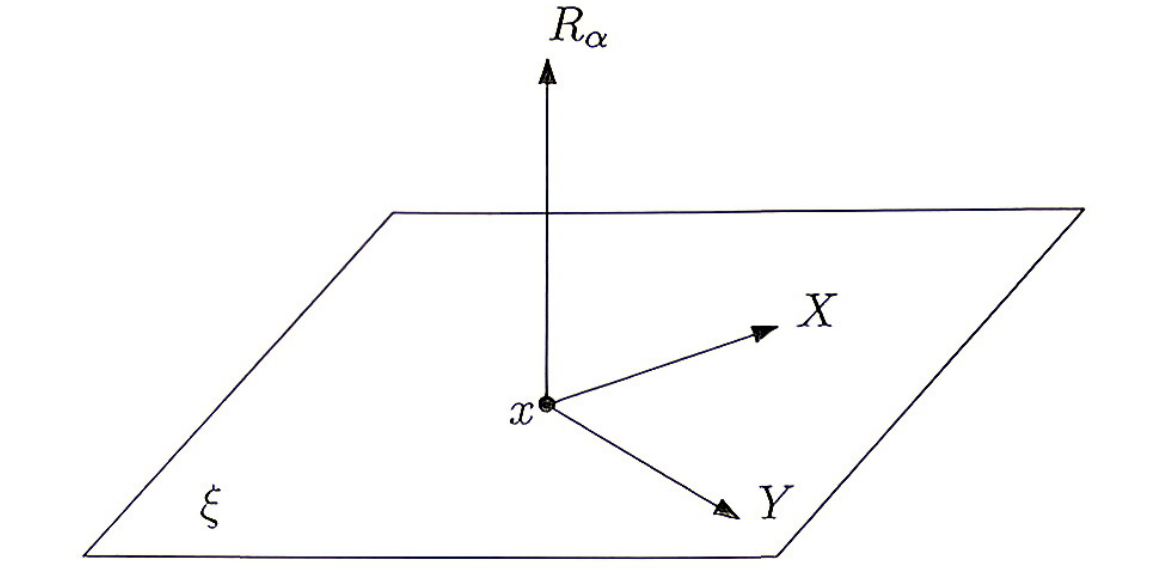
\includegraphics[width=0.52\linewidth]{figures/fig_p063_1.png}
  \caption*{图 3.1\quad Reeb 向量场 $R_\alpha$ 与 $\xi$ 横截
  （原书 p.55, Figure 3.1）}
\end{figure}
